%----------------------------------------------------------------------------------------
%	PACKAGES AND OTHER DOCUMENT CONFIGURATIONS
%----------------------------------------------------------------------------------------

\documentclass[12pt]{article}
\usepackage[danish]{babel}
\usepackage{mathtools}
\usepackage[euler]{textgreek}
\usepackage[numbered,final]{mcode}
\usepackage[utf8x]{inputenc}
\usepackage{amsmath}
\usepackage{graphicx}
\usepackage[colorinlistoftodos]{todonotes}
\usepackage[toc,page]{appendix}
%\usepackage{float}
\usepackage{floatrow} % used for adding "Source" to pictures
\usepackage{hyperref} % used for hyperlinks
\usepackage[all]{hypcap}
 \usepackage{bm} % used for bold inline matj
\usepackage{lipsum} % used for lorem lipsum
\usepackage[final]{pdfpages} % used for including PDF's
\usepackage{geometry}
\usepackage{listingsutf8}
\usepackage{listings}
\usepackage{color} %red, green, blue, yellow, cyan, magenta, black, white
\definecolor{mygreen}{RGB}{28,172,0} % color values Red, Green, Blue
\definecolor{mylilas}{RGB}{170,55,241}

\hypersetup{colorlinks=true, linkcolor=black}

% Page margins
\geometry{verbose,tmargin=1in,bmargin=1in,lmargin=1in,rmargin=1in,headsep=0.35in}

\begin{document}
	
	\begin{titlepage}
		
		
		
		\newcommand{\HRule}{\rule{\linewidth}{0.5mm}} % Defines a new command for the horizontal lines, change thickness here
		\setlength{\topmargin}{0in}
		\centering % Center everything on the page
		
		%----------------------------------------------------------------------------------------
		%	HEADING SECTIONS
		%----------------------------------------------------------------------------------------
		\textsc{\LARGE Aarhus universitet}\\[1.5cm] % Name of your university/college
		\textsc{\Large Anvendte Microcontroller Systemer}\\[0.5cm] % Major heading such as course name
		\textsc{\large 6. Semester}\\[0.5cm] % Minor heading such as course title
		
		%----------------------------------------------------------------------------------------
		%	TITLE SECTION
		%----------------------------------------------------------------------------------------
		
		\HRule \\[0.4cm]
		{ \huge \bfseries AMS projekt}\\ % Title of your document
		\HRule \\[1cm]
		
		%----------------------------------------------------------------------------------------
		%	AUTHOR SECTION
		%----------------------------------------------------------------------------------------
		
		\begin{minipage}{0.4\textwidth}
			\begin{flushleft} \large
				\emph{Gruppemedlemmer:}\\
				Søren Landgrebe \\
				Philip Nygaard Scmhidt \\
			\end{flushleft}
		\end{minipage}
		~
		\begin{minipage}{0.4\textwidth}
			\begin{flushright} \large
				\emph{Studienr:} \\
				201508295\\
				201401682\
			\end{flushright}
		\end{minipage}\\[5cm]
		
		%----------------------------------------------------------------------------------------
		%	LOGO SECTION
		%----------------------------------------------------------------------------------------
		
		
\includegraphics[scale=0.5]{Img/logo.jpg}\\[1cm]
		
		%----------------------------------------------------------------------------------------
		%	DATE SECTION
		%----------------------------------------------------------------------------------------
		
		{\large \today}\\[0.5cm] % Date, change the \today to a set date if you want to be precise
		
		
		\vfill % Fill the rest of the page with whitespace
		
	\end{titlepage}
	
\newpage
\tableofcontents
\newpage
\listoffigures
\newpage

\hypersetup{linkcolor=blue}



%!TEX root = ../../Main.tex
\graphicspath{{Chapters/Indledning/}}
%-------------------------------------------------------------------------------

\section{Indledning}
Næsten alle danskere har nu til dags en smartphone med indbygget Bluetooth modul, som man altid har med på sig, når man forlader sit hjem. Dette vil gruppen gerne udnytte til at kunne gøre det nemmere for brugere, at kunne låse op og låse hoveddøren, som adskiller omverdenen fra ens dyrebare ejendele. Dette betyder at forbrugeren aldrig skal tænke mere på nøgler, da disse bliver overflødige. Hermed slipper brugeren for at skulle huske på dette, samt at skulle fumle med nøglerne når man kommer hjem med flere poser i hænderne fra dagens indkøbstur. 

\begin{figure}[H]
	\centering
	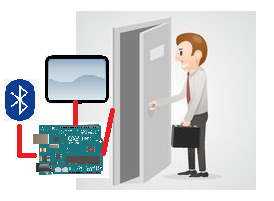
\includegraphics[width = 300 pt]{Img/Konceptbillede.png}
	\caption{Konceptbillede}
	\label{fig:Konceptbillede}
\end{figure}

	%!TEX root = ../../Main.tex
\graphicspath{{Chapters/Krav/}}
%-------------------------------------------------------------------------------


\section{Krav}
I dette afsnit beskrives kravene til hvilken funktionalitet systemet har. 


I samarbejde med vejleder er der opstillet en række krav.
\begin{itemize}
\item Systemet skal kunne finde de 4 stærkeste bluetooth signaler. 
\item Systemet skal kunne køre "hele tiden"
\item Systemet skal opdateres en gang i hvert sekund.  
\end{itemize}


%!TEX root = ../../Main.tex
\graphicspath{{Chapters/Struktur/}}
%-------------------------------------------------------------------------------

\section{Graphic display driver}

Som brugergrænseflade i dette projekt bruges et ITDB02, som er valgt da der tidligere er arbejdet med netop dette produkt. Dertil kommer ILI9341 som driver til selve display'et. 

Driver softwaren til hele displayet, er delt op i flere forskellige cpp filer, dette er gjort for at gøre koden mere overskuelig, og gøre funktionaliteten mere effektiv. Herunder forsøges at gøre et overblik over de forskellige cpp filer og deres integeren. 


\begin{figure}[H]
	\centering
	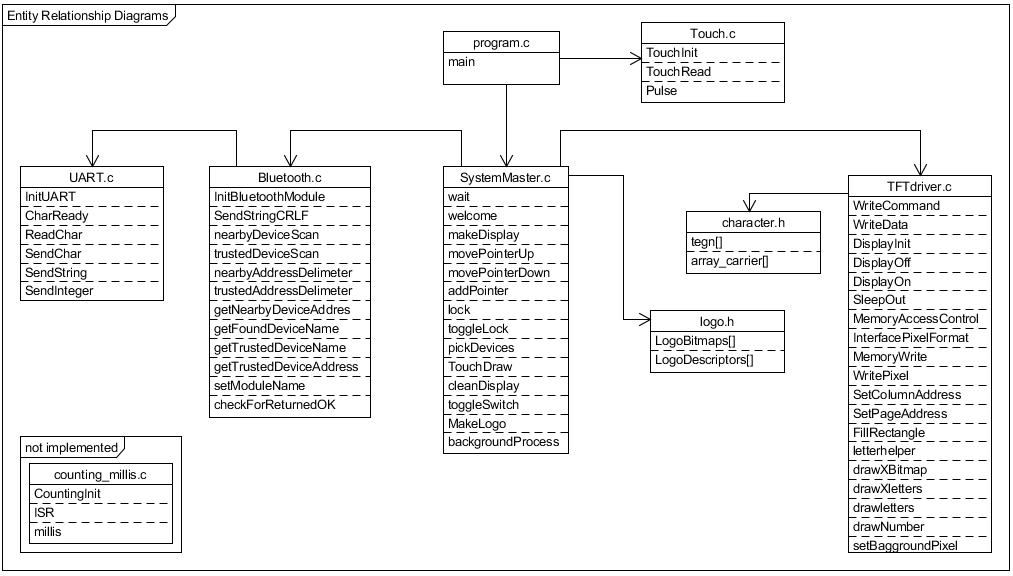
\includegraphics[width = 300 pt]{Img/Entity.png}
	\caption{Entity Relationship Diagrams}
	\label{fig:Konceptbillede}
\end{figure}
 
---Skriv noget når det hele er færdig her




%!TEX root = ../../Main.tex
\graphicspath{{Chapters/Indledning/}}
%-------------------------------------------------------------------------------


\section{Teori}
I procceseringsfasen af projektet, har vi valgt at bruge et adaptivt filter - LMS (Least Mean square) algoritme. LMS er et adaptivt filter som består af 2 funktionelle blokke, hvor den ene blok (Linear Filter) fungerer som et filter, det andet (Adaptive Algorithm) som et dynamisk beregner af nye koefficinter til første blok.  Filteret trækker herefter de beregnede filter fra det samlede lydsignal. 
   

\begin{figure}[H]
	\centering
	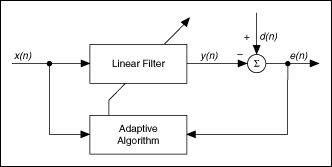
\includegraphics[width = 400pt]{Img/Figures}
	\caption{LMS adaptive filter}
	\label{fig:LMS_filter}
\end{figure}

På figur \ref{fig:LMS_filter} ses et overblik over det adative system, hvor x(n) er støjsignalet, y(n) er det filtrede støjsignal, med koefficienter som opdateres fra blokken "Adaptive Algoritm". d(n) er det ønskede signal inklusiv det støjende signal. e(n) er forskellen mellem d(n) og y(n) og derved støjen fratrukket fra det samlede signal af ønsket og støj.\cite{Teori}  \newline 


Det digitale filter bliver beregnet ud fra formlen:

\begin{equation}
  y(n) = \displaystyle\sum_{l=0}^{L-1} W(n)*x(n-1)
\end{equation}
Hvor W(n) er den værdi, som dynamisk opdateres. Dette sker ved at vi beregner den næste værdi ud fra formlen: 

\begin{equation}
  W(n+1) = W(n)-\mu *X(n)*e(n)
\end{equation}

Hvor W er den nye koefficient til filteret, X(n) er input signalet, og \textmu\ er en faktor, som bestemmer hastigheden af filteret, samt styrer infaldstiden. Hvis \textmu\ er lav bliver filteret langtsommere, mens settling time stiger jo højere vi kommer. Typisk må denne værdi ikke overstige 1. 
\newline
Dette giver os et endeligt udtryk som stemmer overens med figur \ref{fig:LMS_filter}, ift summeringspunktet: 
\begin{equation}
  e(n) = d(n)-y(n)
\end{equation} 


\begin{flushleft}
	
\end{flushleft}


\bibliographystyle{plain}
\bibliography{Bibliography}	

\begin{thebibliography}{9}

\bibitem{Teori} 
Gan and Kuo. \\
\textit{Embedded Signal Processing with the Micro Signal Architecture, Chapter 4.4.1}\\ 
John Wiley 1st Ed. 2007.
 
\bibitem{Struktur} 
Gan and Kuo. \\
\textit{Embedded Signal Processing with the Micro Signal Architecture, Chapter 7.2.2.1}\\ 
John Wiley 1st Ed. 2007.
  
\end{thebibliography}

\end{document}